\chapter{Subgraph equations}\label{subgraph-eq}

In this project we study the 4694 equational laws (up to symmetry and relabeling) that involve at most four applications of the binary operation $\circ$.  The full list of such laws may be found \href{https://github.com/teorth/equational_theories/blob/main/equational_theories/AllEquations.lean}{here}, and a script for generating them may be found \href{https://github.com/teorth/equational_theories/blob/main/scripts/generate_eqs_list.py}{here}.  The list is sorted by the total number of operations, then by the number of operations on the LHS. Within each such class we define an order on expressions by variable $<$ operation, and lexical order on variables.

Selected equations of interest are listed below, as well as in \href{https://github.com/teorth/equational_theories/blob/main/equational_theories/Equations.lean}{this file}.  Equations in this list will be referred to as ``subgraph equations'', as we shall inspect the subgraph of the implication subgraph induced by these equations.




\begin{definition}[Equation 1]\label{eq1}\lean{Equation1}\leanok\uses{magma-def}  Equation 1 is the law $x=x$.
\end{definition}

This is the trivial law, satisfied by all magmas. It is self-dual.


\begin{definition}[Equation 2]\label{eq2}\lean{Equation2}\leanok\uses{magma-def}  Equation 2 is the law $x=y$.
\end{definition}

This is the singleton law, satisfied only by the empty and singleton magmas.  It is self-dual.

\begin{definition}[Equation 3]\label{eq3}\lean{Equation3}\leanok\uses{magma-def}  Equation 3 is the law $x=x \circ x$.
\end{definition}

This is the idempotence law.  It is self-dual.

\begin{definition}[Equation 4]\label{eq4}\lean{Equation4}\leanok\uses{magma-def}  Equation 4 is the law $x=x \circ y$.
\end{definition}

This is the left absorption law.

\begin{definition}[Equation 5]\label{eq5}\lean{Equation5}\leanok\uses{magma-def}  Equation 5 is the law $x=y \circ x$.
\end{definition}

This is the right absorption law (the dual of Definition \ref{eq4}).

\begin{definition}[Equation 6]\label{eq6}\lean{Equation6}\leanok\uses{magma-def}  Equation 6 is the law $x=y \circ y$.
\end{definition}

This law is equivalent to the singleton law.

\begin{definition}[Equation 7]\label{eq7}\lean{Equation7}\leanok\uses{magma-def}  Equation 7 is the law $x=y \circ z$.
\end{definition}

This law is equivalent to the singleton law.

\begin{definition}[Equation 8]\label{eq8}\lean{Equation8}\leanok\uses{magma-def}  Equation 8 is the law $x=x \circ (x \circ x)$.
\end{definition}

\begin{definition}[Equation 23]\label{eq23}\lean{Equation23}\leanok\uses{magma-def}  Equation 23 is the law $x= (x \circ x) \circ x$.
\end{definition}

This is the dual of Definition \ref{eq8}.

\begin{definition}[Equation 38]\label{eq38}\lean{Equation38}\leanok\uses{magma-def}  Equation 38 is the law $x \circ x = x \circ y$.
\end{definition}

This law asserts that the magma operation is independent of the second argument.

\begin{definition}[Equation 39]\label{eq39}\lean{Equation39}\leanok\uses{magma-def}  Equation 39 is the law $x \circ x = y \circ x$.
\end{definition}

This law asserts that the magma operation is independent of the first argument (the dual of Definition \ref{eq38}).

\begin{definition}[Equation 40]\label{eq40}\lean{Equation40}\leanok\uses{magma-def}  Equation 40 is the law $x \circ x = y \circ y$.
\end{definition}

This law asserts that all squares are constant. It is self-dual.

\begin{definition}[Equation 41]\label{eq41}\lean{Equation41}\leanok\uses{magma-def}  Equation 41 is the law $x \circ x = y \circ z$.
\end{definition}

This law is equivalent to the constant law, Definition \ref{eq46}.

\begin{definition}[Equation 42]\label{eq42}\lean{Equation42}\leanok\uses{magma-def}  Equation 42 is the law $x \circ y = x \circ z$.
\end{definition}

Equivalent to Definition \ref{eq38}.

\begin{definition}[Equation 43]\label{eq43}\lean{Equation43}\leanok\uses{magma-def}  Equation 43 is the law $x \circ y = y \circ x$.
\end{definition}

The commutative law. It is self-dual.

\begin{definition}[Equation 45]\label{eq45}\lean{Equation45}\leanok\uses{magma-def}  Equation 45 is the law $x \circ y = z \circ y$.
\end{definition}

This is the dual of Definition \ref{eq42}.

\begin{definition}[Equation 46]\label{eq46}\lean{Equation46}\leanok\uses{magma-def}  Equation 46 is the law $x \circ y = z \circ w$.
\end{definition}

The constant law: all products are constant. It is self-dual.

\begin{definition}[Equation 168]\label{eq168}\lean{Equation168}\leanok\uses{magma-def}  Equation 168 is the law $x = (y \circ x) \circ (x \circ z)$.
\end{definition}

The law of a central groupoid. It is self-dual.

\begin{definition}[Equation 387]\label{eq387}\lean{Equation387}\leanok\uses{magma-def}  Equation 387 is the law $x \circ y = (y \circ y) \circ x$.
\end{definition}


\begin{definition}[Equation 4512]\label{eq4512}\lean{Equation4512}\leanok\uses{magma-def}  Equation 4512 is the law $x \circ (y \circ z) = (x \circ y) \circ z$.
\end{definition}

The associative law. It is self-dual.

\begin{definition}[Equation 4513]\label{eq4513}\lean{Equation4513}\leanok\uses{magma-def}  Equation 4513 is the law $x \circ (y \circ z) = (x \circ y) \circ w$.
\end{definition}

\begin{definition}[Equation 4522]\label{eq4522}\lean{Equation4522}\leanok\uses{magma-def}  Equation 4522 is the law $x \circ (y \circ z) = (x \circ w) \circ u$.
\end{definition}

Dual to Definition \ref{eq4579}.

\begin{definition}[Equation 4564]\label{eq4564}\lean{Equation4564}\leanok\uses{magma-def}  Equation 4564 is the law $x \circ (y \circ z) = (w \circ y) \circ z$.
\end{definition}

Dual to Definition \ref{eq4513}.

\begin{definition}[Equation 4579]\label{eq4579}\lean{Equation4579}\leanok\uses{magma-def}  Equation 4579 is the law $x \circ (y \circ z) = (w \circ u) \circ z$.
\end{definition}

Dual to Definition \ref{eq4522}.

\begin{definition}[Equation 4582]\label{eq4582}\lean{Equation4582}\leanok\uses{magma-def}  Equation 4582 is the law $x \circ (y \circ z) = (w \circ u) \circ v$.
\end{definition}

This law asserts that all triple constants (regardless of bracketing) are constant.

Implications between these laws are depicted in Figure \ref{fig:implications}.

\begin{figure}
  \centering
  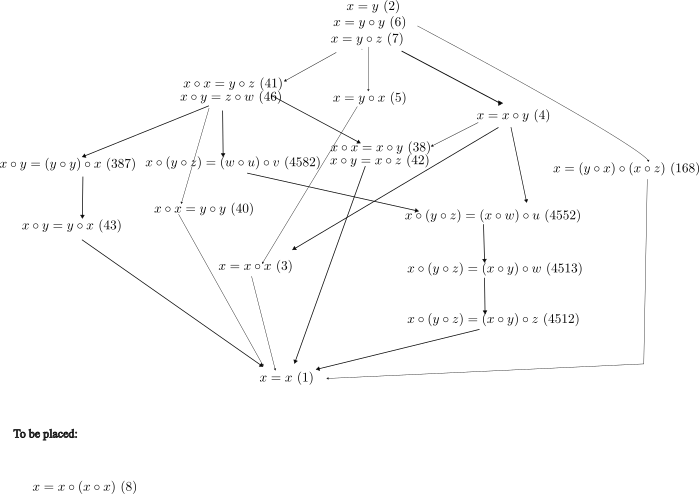
\includegraphics[width=0.5\linewidth]{../../images/implications.png}
  \caption{Implications between the above equations.}
  \label{fig:implications}
\end{figure}
